\begin{frame}
\frametitle{Tipo de soluciones}

Algoritmo:
\begin{block}{Definición (usada en este trabajo)}
 Un algoritmo es cualquier procedimiento bien
definido que toma algún valor, o conjunto de valores como entrada
(o \textbf{Input}) y produce algún valor, o conjunto de valores como
salida (u \textbf{Output}). Un algoritmo siempre termina.
\end{block}

\pause

Ejemplos: 

\begin{itemize}
\item Suma de los primeros $n \in \mathbb{N}$ ($O(n)$).
\item Mergesort ($O(n\log(n))$).
\item Algoritmo de Dijkstra ($O(|E| + |V|\log(|V|))$).
\end{itemize}

\pause

\begin{itemize}
		\item[$\blacksquare$] Ventaja: Garantía de resultado.
		\item[$\blacksquare$] Desventaja: Tiempo poco realista en problemas $\notin$ \textsl{P}.
\end{itemize}

\end{frame}


\begin{frame}
\frametitle{Algoritmos fuera de la clase \textsl{P}}

\begin{block}{3-SAT}
Dado un conjunto de fórmulas
$\phi = \{x_{1}, x_{2}, x_{3}, ..., x_{n}\}$ con cada $x_{i}$ una fórmula lógica
de la forma $x_{i} = p_{i} \lor q_{i} \lor r_{i} $, con $ p_{i}, q_{i}, r_{i}$,
variables o términos lógicos, se deberá encontrar una
interpretación $\mathcal{I}$ tal que $\mathcal{I}(\phi) = \mathcal{I}(x_{i}) = 1$
$\forall i \in \{1,2,...,n\}$.
\end{block}
\pause
¿Qué pasa si aplicamos un algoritmo para encontrar la solución de un problema como \texttt{3-SAT} $\in$ \textsl{NP}-completo?

\begin{columns}
\column{0.5\textwidth}
\begin{figure}[h]
\scalebox{.4}{% GNUPLOT: LaTeX picture
\setlength{\unitlength}{0.240900pt}
\ifx\plotpoint\undefined\newsavebox{\plotpoint}\fi
\sbox{\plotpoint}{\rule[-0.200pt]{0.400pt}{0.400pt}}%
\begin{picture}(1500,900)(0,0)
\sbox{\plotpoint}{\rule[-0.200pt]{0.400pt}{0.400pt}}%
\put(171.0,131.0){\rule[-0.200pt]{4.818pt}{0.400pt}}
\put(151,131){\makebox(0,0)[r]{$0$}}
\put(1419.0,131.0){\rule[-0.200pt]{4.818pt}{0.400pt}}
\put(171.0,313.0){\rule[-0.200pt]{4.818pt}{0.400pt}}
\put(151,313){\makebox(0,0)[r]{$500$}}
\put(1419.0,313.0){\rule[-0.200pt]{4.818pt}{0.400pt}}
\put(171.0,495.0){\rule[-0.200pt]{4.818pt}{0.400pt}}
\put(151,495){\makebox(0,0)[r]{$1,000$}}
\put(1419.0,495.0){\rule[-0.200pt]{4.818pt}{0.400pt}}
\put(171.0,677.0){\rule[-0.200pt]{4.818pt}{0.400pt}}
\put(151,677){\makebox(0,0)[r]{$1,500$}}
\put(1419.0,677.0){\rule[-0.200pt]{4.818pt}{0.400pt}}
\put(171.0,859.0){\rule[-0.200pt]{4.818pt}{0.400pt}}
\put(151,859){\makebox(0,0)[r]{$2,000$}}
\put(1419.0,859.0){\rule[-0.200pt]{4.818pt}{0.400pt}}
\put(171.0,131.0){\rule[-0.200pt]{0.400pt}{4.818pt}}
\put(171,90){\makebox(0,0){$2$}}
\put(171.0,839.0){\rule[-0.200pt]{0.400pt}{4.818pt}}
\put(488.0,131.0){\rule[-0.200pt]{0.400pt}{4.818pt}}
\put(488,90){\makebox(0,0){$3$}}
\put(488.0,839.0){\rule[-0.200pt]{0.400pt}{4.818pt}}
\put(805.0,131.0){\rule[-0.200pt]{0.400pt}{4.818pt}}
\put(805,90){\makebox(0,0){$4$}}
\put(805.0,839.0){\rule[-0.200pt]{0.400pt}{4.818pt}}
\put(1122.0,131.0){\rule[-0.200pt]{0.400pt}{4.818pt}}
\put(1122,90){\makebox(0,0){$5$}}
\put(1122.0,839.0){\rule[-0.200pt]{0.400pt}{4.818pt}}
\put(1439.0,131.0){\rule[-0.200pt]{0.400pt}{4.818pt}}
\put(1439,90){\makebox(0,0){$6$}}
\put(1439.0,839.0){\rule[-0.200pt]{0.400pt}{4.818pt}}
\put(171.0,131.0){\rule[-0.200pt]{0.400pt}{175.375pt}}
\put(171.0,131.0){\rule[-0.200pt]{305.461pt}{0.400pt}}
\put(1439.0,131.0){\rule[-0.200pt]{0.400pt}{175.375pt}}
\put(171.0,859.0){\rule[-0.200pt]{305.461pt}{0.400pt}}
\put(30,495){\rotatebox{90}{\makebox(0,0){Asignaciones}}
}\put(805,29){\makebox(0,0){Fórmulas}}
\put(488,136){\usebox{\plotpoint}}
\multiput(488.00,136.58)(3.894,0.498){79}{\rule{3.193pt}{0.120pt}}
\multiput(488.00,135.17)(310.373,41.000){2}{\rule{1.596pt}{0.400pt}}
\multiput(805.58,177.00)(0.500,0.514){631}{\rule{0.120pt}{0.511pt}}
\multiput(804.17,177.00)(317.000,324.939){2}{\rule{0.400pt}{0.256pt}}
\put(488,136){\makebox(0,0){$+$}}
\put(805,177){\makebox(0,0){$+$}}
\put(1122,503){\makebox(0,0){$+$}}
\put(1122.0,503.0){\rule[-0.200pt]{0.400pt}{85.760pt}}
\put(171.0,131.0){\rule[-0.200pt]{0.400pt}{175.375pt}}
\put(171.0,131.0){\rule[-0.200pt]{305.461pt}{0.400pt}}
\put(1439.0,131.0){\rule[-0.200pt]{0.400pt}{175.375pt}}
\put(171.0,859.0){\rule[-0.200pt]{305.461pt}{0.400pt}}
\end{picture}
}
\end{figure} 

\column{0.5\textwidth}
\begin{figure}
\scalebox{.4}{\begin{figure}[H]
\centering
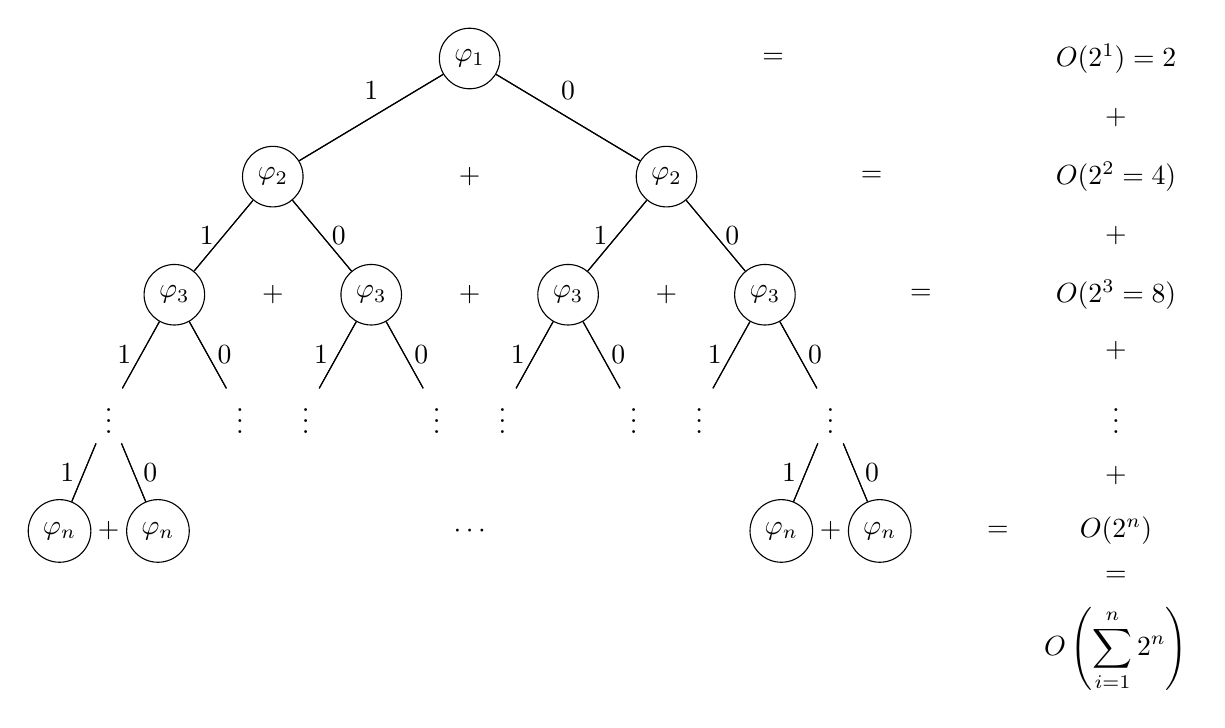
\begin{tikzpicture}[level/.style={sibling distance=50mm/#1}]
\node [circle,draw] (z){$\varphi_{1}$}
  child {node [circle,draw] (a) {$\varphi_{2}$}
    child {node [circle,draw] (b) {$\varphi_{3}$}
      child {node (p1) {$\vdots$}
        child {node [circle,draw] (d) {$\varphi_{n}$}}
        child {node [circle,draw] (e) {$\varphi_{n}$}}
      }
      child {node (p2) {$\vdots$}}
    }
    child {node [circle,draw] (g) {$\varphi_{3}$}
      child {node (p3) {$\vdots$}}
      child {node (p4) {$\vdots$}}
    }
  }
  child {node [circle,draw] (j) {$\varphi_{2}$}
    child {node [circle,draw] (k) {$\varphi_{3}$}
      child {node (p5) {$\vdots$}}
      child {node (p6) {$\vdots$}}
    }
  child {node [circle,draw] (l) {$\varphi_{3}$}
    child {node (p7) {$\vdots$}}
    child {node (c){$\vdots$}
      child {node [circle,draw] (o) {$\varphi_{n}$}}
      child {node [circle,draw] (p) {$\varphi_{n}$}
        child [grow=right] {node (q) {$=$} edge from parent[draw=none]
          child [grow=right] {node (q) {$O(2^{n})$} edge from parent[draw=none]
            child [grow=up] {node (r) {$\vdots$} edge from parent[draw=none]
              child [grow=up] {node (s) {$O(2^{3}=8)$} edge from parent[draw=none]
                child [grow=up] {node (t) {$O(2^{2}=4)$} edge from parent[draw=none]
                  child [grow=up] {node (u) {$O(2^{1})=2$} edge from parent[draw=none]}
                }
              }
            }
            child [grow=down] {node (v) {$O\left(\displaystyle\sum_{i = 1}^n 2^n \right)$}edge from parent[draw=none]}
          }
        }
      }
    }
  }
};
\path (a) -- (j) node [midway] {+};
\path (b) -- (g) node [midway] {+};
\path (k) -- (l) node [midway] {+};
\path (k) -- (g) node [midway] {+};
\path (d) -- (e) node [midway] {+};
\path (o) -- (p) node [midway] {+};
\path (o) -- (e) node (x) [midway] {$\cdots$};
\path (q) -- (r) node [midway] {+};
\path (s) -- (r) node [midway] {+};
\path (s) -- (t) node [midway] {+};
\path (s) -- (l) node [midway] {=};
\path (t) -- (u) node [midway] {+};
\path (z) -- (u) node [midway] {=};
\path (j) -- (t) node [midway] {=};
\path (q) -- (v) node [midway] {=};



\path (z) edge node[above=3pt]{$1$} (a);
\path (z) edge node[above=3pt]{$0$} (j);

\path (a) edge node[left]{$1$} (b);
\path (a) edge node[right]{$0$} (g);
\path (j) edge node[left]{$1$} (k);
\path (j) edge node[right]{$0$} (l);

\path (b) edge node[left]{$1$} (p1);
\path (b) edge node[right]{$0$} (p2);
\path (g) edge node[left]{$1$} (p3);
\path (g) edge node[right]{$0$} (p4);
\path (k) edge node[left]{$1$} (p5);
\path (k) edge node[right]{$0$} (p6);
\path (l) edge node[left]{$1$} (p7);
\path (l) edge node[right]{$0$} (c);

\path (p1) edge node[left]{$1$} (d);
\path (p1) edge node[right]{$0$} (e);
\path (c) edge node[left]{$1$} (o);
\path (c) edge node[right]{$0$} (p);

\end{tikzpicture}
\caption{Posibles valores de verdad por cada variable en un árbol binario.} \label{fig:a3sat02}
\end{figure}}
\end{figure}

\end{columns}
\end{frame}